\chapter{Te\'{o}ria}
\label{ch:theory}

V tejto kapitole sa budeme venovať teórii stojacej v pozadí programovanej aplikácie.
Vysvetlíme si algoritmy na rozdelenie práce v distribuovanom prostredí, predstavíme
si algoritmy vytvárania a prechádzania grafu závislostí, ktoré sú neoddeliteľnou
súčasťou každého build systému.

\section{Graf cie\v{l}ov}
\label{sec:depgraph}

Jednou z neoddeliteľných súčastí akéhokoľvek väčšieho projektu je používanie knižníc
na poskytovanie funkcionality, ktorú projekt požaduje. Typickými príkladmi je spracovávanie
testových alebo binárnych formátov ako JSON alebo YAML, alebo komunikácia cez sieť.

Pre svoju úspešnú kompiláciu projekt vyžaduje, aby tieto knižnice, na ktorých závisí,
boli dostupné, častokrát už v skompilovanej podobne, na kompilujúcom počítači. Takéto
knižnice nazývame závislosťami projektu a v BUILD súboroch ich uvádzame, ako ciele
kompilácie v zozname dependencies, z anglického termínu pre závislosť.

Naša aplikácia pri spustení prejde rekurzívne definície vyžiadaných cieľov a ich závislostí,
pričom vytvára orientovaný graf, tzv.\ graf cieľov. Pre tento graf vyžadujeme, aby bol
acyklický. V opačnom prípade nevieme splniť požiadavky cieľa, ktorý obsahuje danú
cyklickú závislosť.

Po vytvorení tohto grafu je tento prejdený od listov nahor. Listy grafu cieľov
sme definovali ako ciele, ktoré nemajú žiadne závislosti a sú teda koncovými uzlami
grafu. Každý z cieľov grafu je následne splnený. V prípade úspešného splnenia cieľa vyžiadaného
používateľom je celá kompilácia ukončená úspechom. Príklad grafu uvázame na obrázku~\ref{img:depgraphtheory}.

\begin{figure}[h]
  \centerline{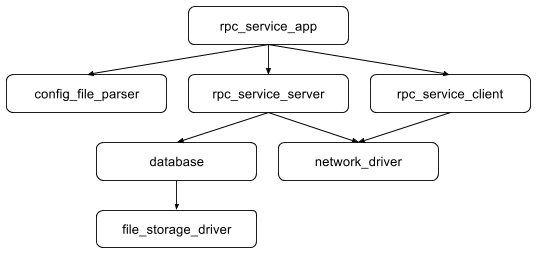
\includegraphics[width=0.8\textwidth]{images/dependency_targets}}
  \caption[Graf cieľov]{Príklad grafu cieľov pre aplikáciu zloženú z RPC servera a klienta}
  \label{img:depgraphtheory}
\end{figure}

\section{Algoritmus distrib\'{u}cie akci\'{i}}
\label{sec:actiondistrib}

Dôležitou časťou akéhokoľvek distribuovaného systému je rozdelenie úloch pre jednotlivé
komponenty. V našej aplikácii sme na tento účel vytvorili Master komponent, ktorý
je spustený používateľom. Master komponent na rozdelenie úloh používa prioritnú radu
(priority queue). Pre každý zo Slave komponentov si udržujeme zoznam súborov, ktoré
daný Slave komponent má k dispozícii, následne spočítame, koľko zo súborov, ktoré
sú potrebné na kompiláciu sú pre každý zo serverov dostupné. K tomuto skóre pripočítame
aktuálne voľný počet pracovných vlákien (v prípade, že počet voľných vlákien je 0, špecifikujeme
  výsledné skóre na 0). Následne akciu pošleme na server s najvyšším skóre.
